\documentclass[a4,12pt]{scrartcl}

%Basic 
\usepackage[utf8]{inputenc}
\usepackage[ngerman]{babel}
\usepackage[T1]{fontenc}
%Schrift 
%\usepackage{fontspec} 
%\setmainfont{Arial} 
%Zeilenabstand
\usepackage{setspace}
\setstretch {1.3}
\usepackage{float}
\usepackage[bottom = 3.50cm]{geometry}

%Titel Seite
\usepackage{titling} %Wird benötigt damit \maketitle die Variabeln title, author und date nicht überschreibt
\title{Test Cases}
\subtitle{Projekt: software name}
\author{David Meister \and Andreas Stalder}		
 %mit /and können Personen hinzugefügt werden
\date{\today}


%Kopf, Fusszeile
\usepackage{fancyhdr}
\pagestyle{fancy}
\lhead{}
\chead{}
\rhead{software name}
\lfoot{\thetitle \: v1.0 }
\cfoot{\today }
\rfoot{Seite \thepage}
\renewcommand{\headrulewidth}{0.4pt}

%Bilder
\usepackage{graphicx}

%Zeichnen
\usepackage{tikz}

%Tabellen
\usepackage{booktabs}
\usepackage{longtable}

%Codesnippets
\usepackage{listings}
\lstset{language=java,basicstyle=\footnotesize,frame=single} %backgroundcolor=\color{lightgray}

%Querformat für eine Seite
\usepackage{lscape}
\usepackage{rotating}
\usepackage{pdflscape}

%URL 
\usepackage[colorlinks=true, linkcolor=blue, urlcolor=blue, citecolor=blue]{hyperref}
\urlstyle{same} 


%Loremimpsum
\usepackage{lipsum}



\begin{document}

%\clearpage\maketitle
\begin{titlepage}
	\centering
	\vspace{5cm}
	\begin{center}
%	\includegraphics[width=0.50\textwidth]{}
	\end{center}
	{\huge\bfseries software name\par}
	\vspace{8cm}
	\raggedright
	{\bfseries HSR Studienarbeit Network Unit Testing\par}
	{\huge\bfseries Network testing\par}
	\vspace{1cm}
	{\theauthor \par}
	{\today\par}

\end{titlepage}

\section{Änderungsgeschichte}

\begin{table}[htb]
\centering
    \begin{tabular}{@{} l l l l@{}}\toprule    
    {Datum} & {Version} & {Änderung} & {Autor}\\ \midrule
    27.09.16 & 1.0 & Erstellung erster Version & dm/as\\ \addlinespace
    \end{tabular}
\caption{\textbf{Änderungsgeschichte}}
\end{table}

\newpage

%\thispagestyle{empty}
\tableofcontents
\newpage


\section{Einführung}
\subsection{Zweck}
Dieses Dokument stellt den Projektplan für unser Studienarbeit dar, es dient zur Planung, Steuerung und Kontrolle.
\subsection{Gültigkeitsbereich}
Dieses Dokument ist über die gesamte Projektdauer gültig. Es wird in späteren Iterationen angepasst. Somit ist jeweils die neuste Version des Dokuments gültig und alte Versionen sind obsolet.
\subsection{Referenzen}
\begin{description}
Noch keine.
%  \item[jNetPcap] \hfill \\
%  \url{http://jnetpcap.com/}
\end{description}

\section{Einleitung}
\subsection{Testing Motivation}
\subsection{}

\section{Device Tests}
\subsection{Scope}
\subsection{Nutzen}
\subsection{Beispiele von Test Cases}
\newpage
\section{Circuit Tests}
\subsection{Scope}
Mit Circuit Tests möchte man die Verbindungen der Devices testen. Mögliche LAN Devices sind unter anderem Access-, Distribution-, und Core Switches, aber auch Router oder Firewalls. Denkbar sind auch Verbindungen im WAN Bereich, ob Ethernet, ATM oder MPLS. Diese Devices haben jeweils unterschiedliche Verbindungen zueinander. Circuit Tests überprüfen Anhand verschiedener Bewertungskriterien die Qualität und Charakteristika dieser Verbindungen.\\

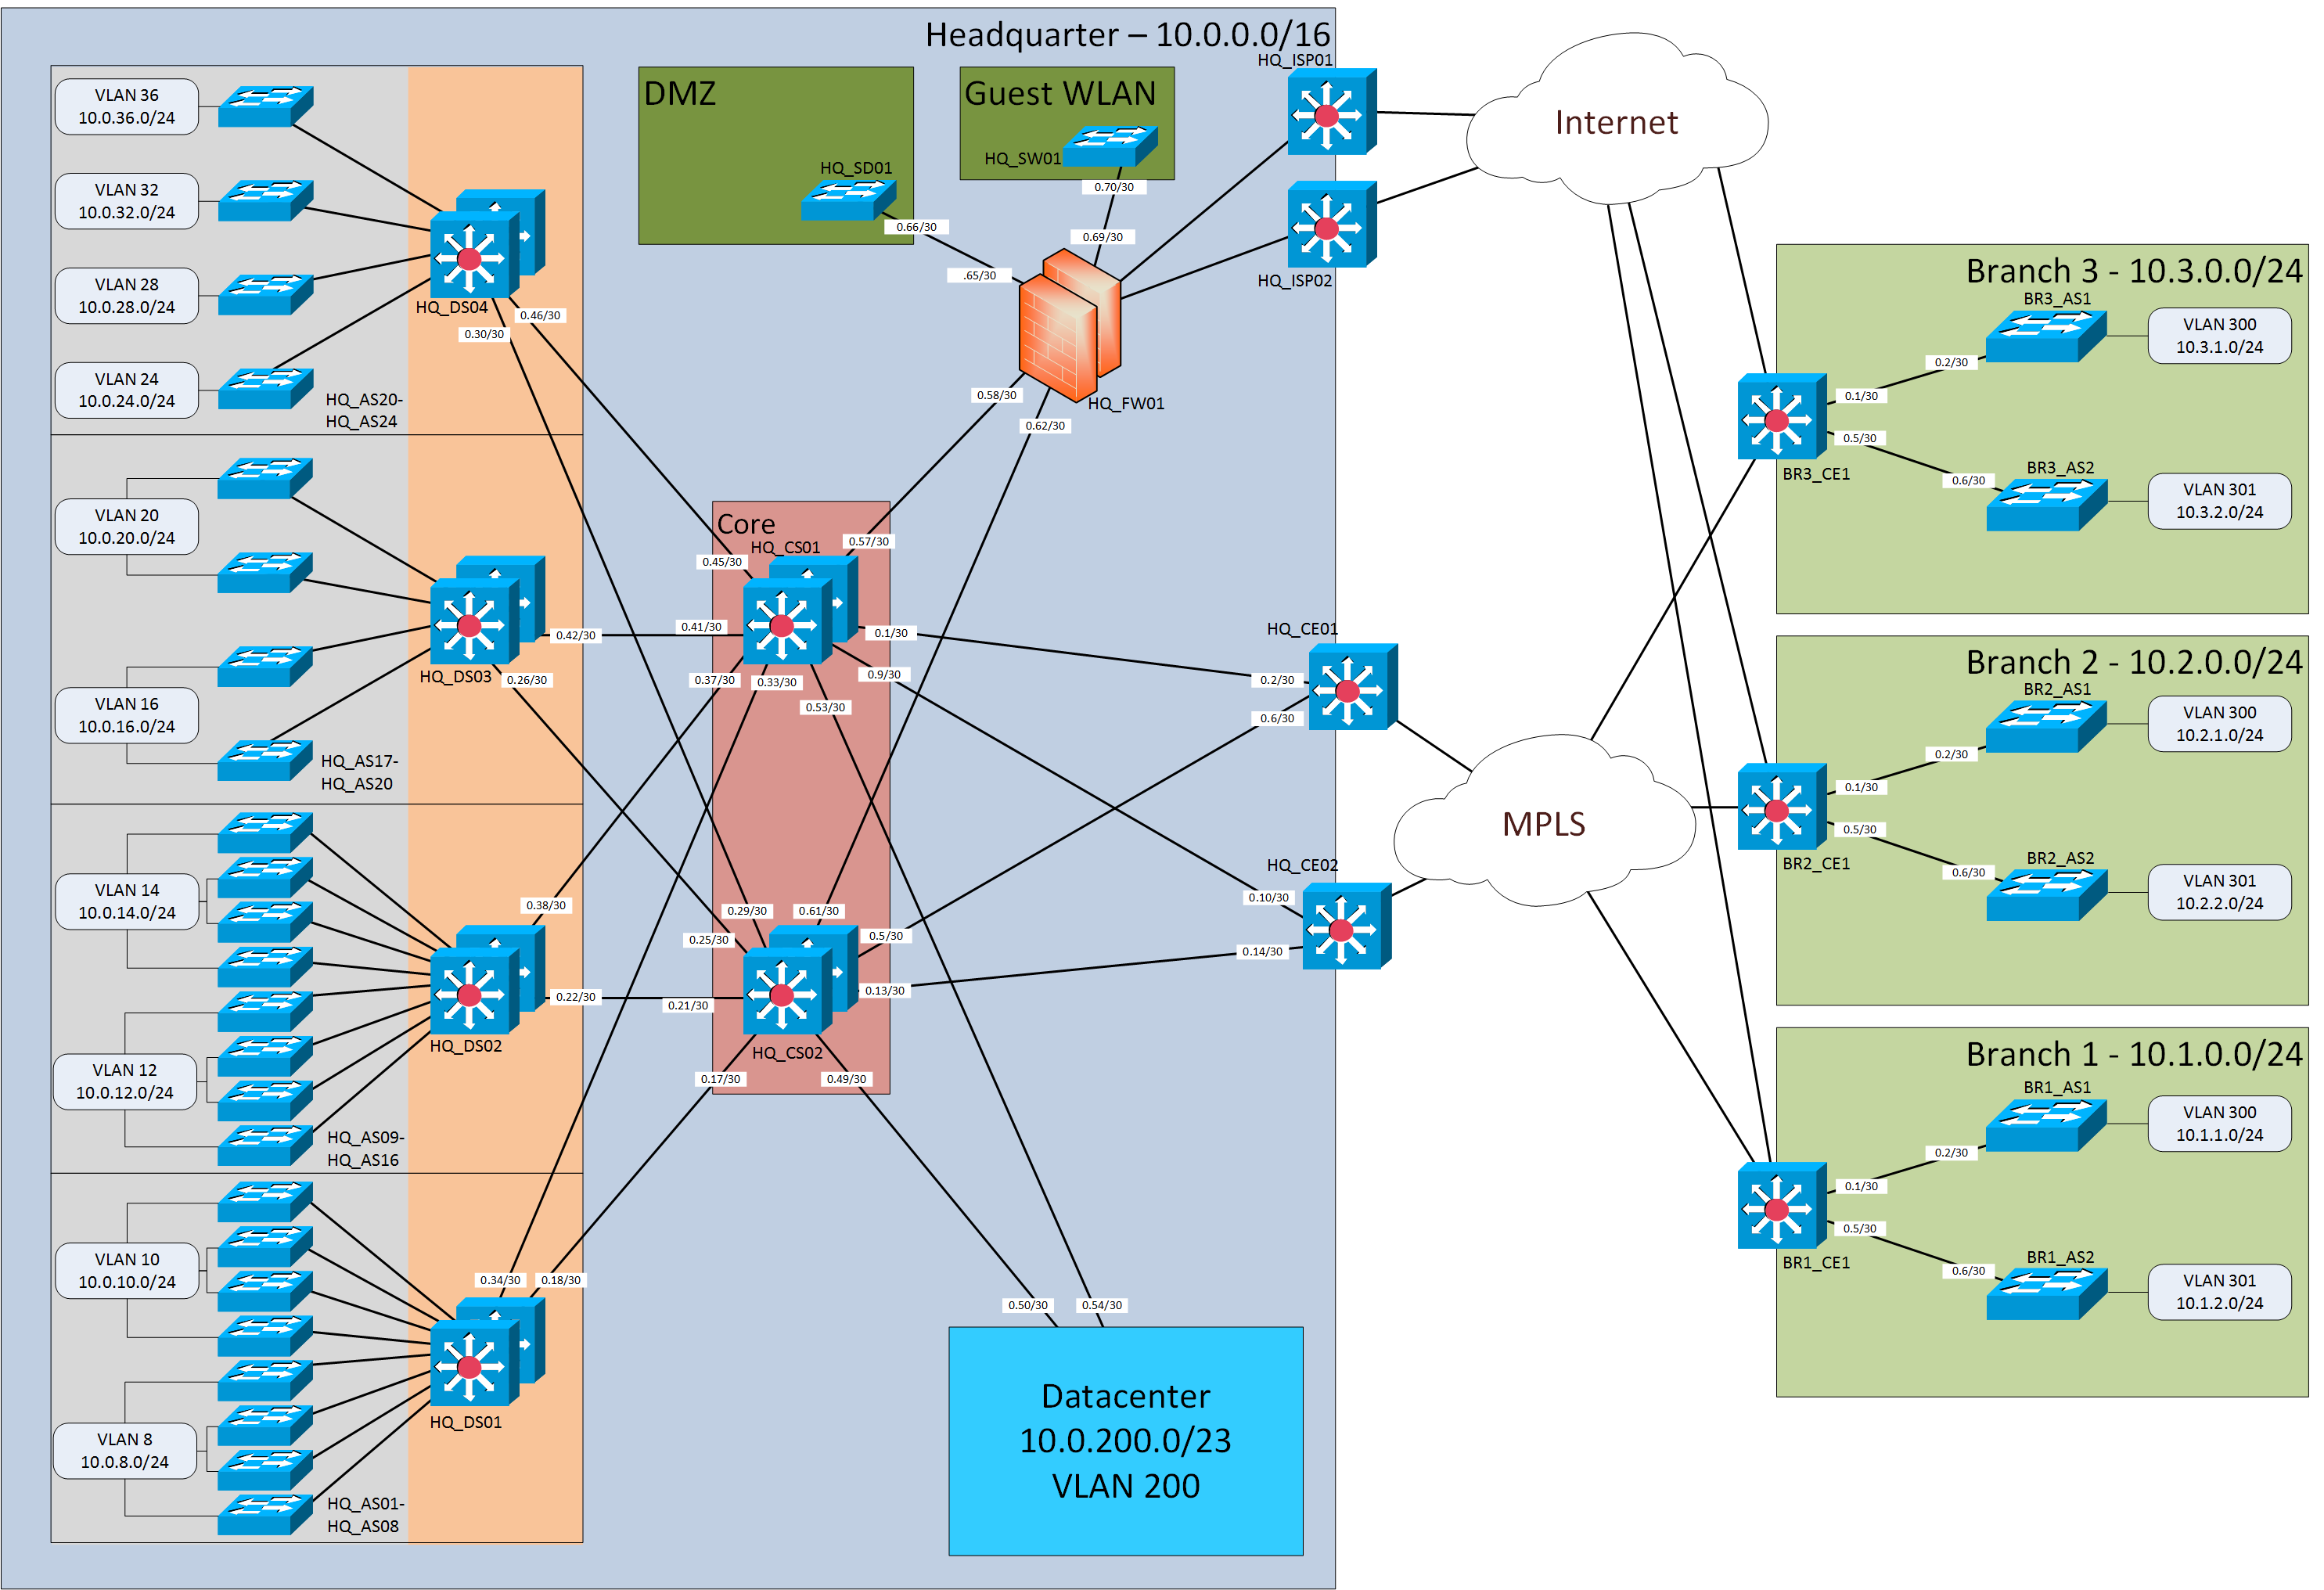
\includegraphics[width=1\textwidth]{figures/Netzwerk_logisch.png}\\

\noindent Wenn von Verbindungsqualität gesprochen wird, möchte man vor allem bestimmte Verbindungsspezifische Parameter wie Round Trip Times, Jitter, Throughput Packet Loss testen. Je nach Verbindung, welche es zu testen gilt, kann man sinnvolle Grenzwerte festlegen. So können gewisse Throughput Werte auf der WAN Verbindung einer Firewall akzeptabel sein, während derselbe Wert auf der LAN Verbindung zu niedrig wäre.\\

\noindent Typischerweise bewegt man sich bei Circuit Tests auf den OSI-Layern 1-3. Es muss jeweils überlegt werden, welche Tests sinnvoll sind, um die komplette Funktionalität der Verbindung auf unterschiedlichen Test Cases abzubilden.   
\subsection{Nutzen}
Durch systematisches Testen der Verbindungen gewinnen wir Vertrauen in die Funktionalität der Verbindungen. Changes im Netzwerk, seien es einfache Konfigurationsänderungen, oder Austausch eines oder mehrerer Devices, können bei auftretenden Fehlern schwerwiegende Folgen mit sich bringen.\\

\noindent Als Verantwortlicher Netzwerk Engineer trägt man eine grosse Verantwortung. Beim unsystematischen ad-hoc Testing werden leider oft essenzielle Funktionen und Parameter nicht getestet. Es wird sich ganz auf das Know-How und die Erfahrung des Verantwortlichen Engineers gestützt. Unter Zeitdruck werden oft nur sehr wenige Tests durchgeführt, bis das Netzwerk wieder für den produktiven Betrieb freigegeben wird. Mit systematischen Circuit Tests werden beispielsweise fehlende Links und Verbindungsfehler auf allen Devices schnell erkannt. 
\subsection{Beispiele von Test Cases}
\subsubsection{Round Trip Time}
Bei der Round Trip Time (RTT) möchte man herausfinden, wieviel Zeit für die Übertragung und Verarbeitung eines Datenpakets über die Verbindung benötigt wird. Da bei den Circuit Tests keine high-level Services getestet werden, sollen Datenpakete gesendet werden, für welche die Gegenstation extrem wenig Zeit benötigt, um diese zu Verarbeiten. Das Interesse besteht also hauptsächlich in der benötigten Zeit für den Übertragungsweg.\\

\noindent Der bekannteste Weg, um die RTT zu ermitteln, ist der ping-Befehl, welcher einen ICMP Request auslöst. Mit Ping kann man die RTT innerhalb der Broadcast Domain, aber auch über dessen Grenzen hinweg ins gesamte Internet herausfinden. Es gibt jedoch noch andere Wege, um die RTT zu bestimmen. Mittels arping wird die RTT über ARP Pakete bestimmt, oder über httping wird die Antwortzeit über das HTTP Protokoll ermittelt. Für Circuit Tests scheint der 'normale' ping über ICMP jedoch der sinnvollste.\\

\noindent Bei der RTT gilt es zu beachten, dass bei zwei Devices $\{a,b\}$ die benötigte Übertragungszeit von a$\rightarrow$b $\neq$ b$\rightarrow$a sein kann. Beim Circuit Testing ist aber eher unwahrscheinlich, dass sich die Latenzzeit der beiden Übertragungswege gross unterscheiden, da in aller Regel in derselben Broadcastdomain oder über sehr wenige Hops getestet wird. Die Einwegs-Latenz ist weitaus aufwändiger zu berechnen, da eine exakte Zeitsynchronisation zwischen a und b stattfinden muss.\\

\noindent Mögliche Einflussgrössen der RTT sind die Distanz, verwendete Kabel, Routing/Switching processing, Queueing Delay oder mögliche Übertragungsfehler. Je nach Anwendungsfall können lange Antwortzeiten einen erheblichen Einfluss auf das Befinden der Netzwerkqualität haben. Besonders heikel sind Anwendungen im Voice oder Video Umfeld. 
\subsubsection{Jitter}
Im Kapitel oben wurde die Funktionsweise, die Ermittlungstechniken, die Einflussgrössen und die Auswirkungen der RTT beschrieben. Im Grunde genommen gilt dies alles auch für den Jitter. Beim Jitter handelt es sich um nichts anderes, als eine statistische Auswertung verschiedenster Antwortzeiten.\\

\noindent Beim Jitter handelt es sich um die Standardabweichung der Antwortzeiten aus einer Menge von Messwerten. Um den Jitterwert einer Verbindung zu bestimmen, benötigen wir also zuerst eine Menge $R = \{r_1,...,r_n\}$ von RTT Messwerten. Nun bestimmen wir den Mittelwert $\mu$ der Messwerte auf der Menge $R$ mittels der Formel $\mu = \frac{r_1+...+r_n}{n}$. Nun können wir mittels der Formel
\begin{equation}
Jitter = \sqrt{\frac{(r_1-\mu)^2 + ... + (r_n-\mu)^2}{n}}
\end{equation}
den endgültigen Jitterwert bestimmen. Hier muss beachtet werden, dass je grösser die Anzahl der Messwerte ist, desto genauer und aussagekräftiger ist auch der resultierende Jitter-Wert.
\\

\noindent Für die Qualität des Netzwerks ist es zum einen wichtig, gute Antwortzeiten auf den Verbindungen zu erhalten, sprich einen guten Mittelwert davon. Entscheidend ist aber auch die Varianz in den Messwerten, da es unbefriedigend scheint, wenn häufig grosse Abweichungen vom Mittelwert entstehen. Daraus könnte resultieren, dass beispielsweise die Sprachqualität eins Telefongesprächs für eine kurze Zeit als gut empfunden wird und etwas später als sehr schlecht.
\subsubsection{Throughput}
Unter Throughput oder Durchsatz wird die Übertragungsrate von Netzwerkpaketen in Bits pro Sekunde (bps) verstanden. Der Durchsatz ist mitunter das wichtigste Merkmal für die Leistungsfähigkeit einer Verbindung. Auf dem Level des Circuit Testings ist man an den Durchsatzraten von den Punkt-zu-Punkt Verbindungen im Netzwerk interessiert. Mit automatischen Throughput Tests können leicht Flaschenhälse im Netzwerk aufgedeckt werden. In einem hierarchisch aufgebauten Netzwerk sind wir in den höheren Schichten auf sehr hohe Datenraten angewiesen, da ansonsten das gesamte Netzwerk extrem verlangsamt wird.\\

\noindent Im Grunde genommen ist der Durchsatz sehr einfach zu ermitteln. Wir müssen von zwei Devices $\{a,b\}$ eine Datenmenge $R_{Bytes}$ senden. Wenn wir also $R$ von $a \rightarrow b$ schicken, so müssen wir bei $b$ die Differenz der Ankunft des ersten Bits $t_0(R)$ zur Ankunft des letzten Bits $t_n(R)$ Messen. Um die Übertragungsrate in bps zu bestimmen rechnen wir
\begin{equation}
Durchsatz = \frac{R_{Bytes} * 8}{t_n(R) - t_0(R)}  
\end{equation} 
Bei Computernetzen rechnen wir, anders als beim Speicherplatz, in 10er Potenzen. Somit entsprechen 1000bps 1kbps und 1000kbps 1mbps usw. Beim Testen des Throughputs muss man jedoch stark auf die Methode achten, mit welcher die Übertragung stattgefunden hat. Je weiter unten man in der ISO/OSI Schicht ist, desto weniger Protokolloverhead fällt bei der Datenübertragung an. Man kann grundsätzlich berechnen, wieviel Overhead dies ist, jedoch kann die Konfiguration der Netzwerkdevices einen Einfluss darauf haben. Beispielsweise kann bei einem Device die Maximum Transfer Unit (MTU) festgesetzt werden. Diese setzt die Rahmengrösse für Layer 2 Pakete fest. Wenn nun die ankommenden Pakete zu gross sind, müssen sie fragmentiert werden. Dadurch würde das das Doppelte an Overhead entstehen.\\

\noindent Wenn wir uns nun Testszenarien von Datenübertragungsraten für Circuit Tests überlegen, so wäre es sinnvoll, alles zu berücksichtigen, was sich auf den Durchsatz auswirken kann. Die Einflussgrössen wären beispielsweise Link Speed, Übertragungsprotokoll, Path MTU, Packet Loss, Dienstgüte (QoS), etc. Aus Sicht der Circuit Tests möchten wir uns noch nicht mit QoS befassen, deshalb achten wir darauf, dass wir möglichst unabhängig von QoS testen können. Grundsätzlich sind wir von allen Verbindungen interessiert, wie schnell sie sind, besonders bei Netzwerkgeräten wie Firewalls, Router, Switches und Servern.\\

\noindent Die meisten Link Speeds werden heutzutage per Auto Negotiation ausgehandelt. Es ist deshalb denkbar, dass bei der Aushandlung etwas schief gegangen ist oder ein Kabel defekt ist. Deshalb können resultierende Link Speeds oder Duplex Modi vom gewünschten Zustand abweichen. Auf sehr performanceintensiven Verbindungen wird häufig auch auf Bündelung von Links (Trunking) zurückgegriffen. Falls einer dieser Links ausfällt, ist es möglich, dass dies gar nie bemerkt wird. Dies ist zwar grundsätzlich die Aufgabe des Monitorings, könnte aber auch mittels eines Tests festgestellt werden. Es ist aber auch möglich, dass der gewählte Load-Balancing Algorithmus nicht funktioniert oder eine ungleiche Lastverteilung verursacht. Mittels eines Tests könnte dies erkannt und gegebenenfalls auf einen anderen Algorithmus zurückgegriffen werden.\\

\noindent
Bei den Throughput Tests im Sinne des Circuit Testings muss darauf geachtet werden, keine Datenübertragungen mit Protokollen von höheren ISO/OSI Schichten durchzuführen. Wir sollten uns vor allem auf Punkt-Punkt Verbindungen (Layer 1 und Layer 2) und Layer 3 Verbindungen über wenige Hops beschränken. So testen wir unter anderem beispielsweise die Datenraten auf dem Uplink vom Distribution- auf den Core-Switch oder vom Access-Switch auf den UC-Server. Auch Tests zwischen unterschiedlichen Netzwerkstandorten wären denkbar. Es ist durchaus interessant zu testen, wie schnell der Durchsatz vom einen Datacenter zum anderen über die MPLS Cloud des Providers ist. Zusammengefasst möchten wir mit den Throughput Tests hier Verbindungen vor allem Punkt-zu-Punkt auf Layer 1 oder Layer 2 überprüfen, aber auch über Broadcastdomänen hinweg in entfernte Subnetze oder Standorte mit dem Ziel, die angestrebten Datenraten auf allen (notwendigen) Links sicherzustellen und mögliche Flaschenhälse im Netzwerk aufzudecken.\\

\noindent Abschliessend gilt für Throughput Tests ganz allgemein anzumerken, dass diese den produktiven Betrieb in erheblichem Masse stören können und keinesfalls leichtfertig ausgeführt werden dürfen. Dies bedarf einer seriösen Zeitplanung und gegebenenfalls Information der Benutzer über mögliche Störungen im Netz.

\subsubsection{Packet Loss} 
Paketverluste können viele Ursachen haben. Manchmal ist ein Paketverlust auch gewollt, beispielsweise bei einer Firewall mittels Drop Policy. In diesem Abschnitt möchten wir uns aber vor allem mit ungewollten Paketverlusten beschäftigen. Diese können beispielsweise bei Fehlern im Übertragungsmedium, oder Überlast eines Routers sein. Die Folgen des Paketverlusts können unterschiedlich sein. Bei TCP Protokollen bewirken Paketverluste Retransmissions, deshalb wird der Durchsatz geringer. Bei Realtime Applikationen wie Video oder VoIP, welche UDP basiert sind, ist ein Qualitätsverlust bemerkbar. Eine gewisse Paketverlustrate ist kaum bemerkbar, aber ab einem gewissen Punkt ist beispielsweise ein Gespräch kaum hörbar.\\

\noindent Packet Loss wird gängigerweise in \% der Gesamtheit angegeben. Um ihn Stichprobenartig zu ermitteln muss man also bei zwei Devices \{a,b\} nur eine gewisse Anzahl Request-Pakete $P$ von $a \rightarrow b$ schicken. Nun Antwortet Station $b$ auf jedes dieser Request Pakete mit einer Response. Station $a$ wiederum vergleicht nun die abgesendete Anzahl an Paketen $P$ mit der erhaltenen Anzahl $P'$. 
Mit der Formel
\begin{equation}
Packet Loss = 1-\frac{P' * 100}{P}
\end{equation}
erhalten wir nun die Paketverlustrate in %.\\

\noindent Man muss unbedingt bedenken, dass der PacketLoss je nach Situation variieren kann. Es ist daher beim Testen wichtig, dass man Unterschiedliche Protokolle und Paketgrössen verwendet um ein aussagekräftiges Ergebnis zu erzielen. Es ist auch denkbar, dass die Paketverlustrate beim Testbetrieb extrem niedrig ist, und wiederum bei Volllast viel höher, dies gilt es ebenfalls zu berücksichtigen. Packet Loss könnte beim ermitteln des Jitters zusätzlich errechnet werden. Ein mächtiges Tool wäre beispielsweise iperf.
\section{Routing Tests}
\subsection{Scope}
\subsection{Nutzen}
\subsection{Beispiele von Test Cases}






\section{Traffic Tests}
\subsection{Scope}
Durch die Traffic Tests kann man den Verkehr auf dem Netzwerk überprüfen. Das heisst es werden wichtige Punkte getestet, die das Verhalten der Pakete im Netzwerk beeinflusst. Wichitg sind vorallem die speziellen Flags, welche die Pakete auf dem Netzwerk erhalten. Dazu gehören insbesondere die QoS und VLAN Flags.\newline
Weiter ist auch der End-to-End Throughput ein wichtiger Teil des Traffic Tests. So kann man über mehrere Netzwerkgeräte hinweg die Geschwindigkeit testen.

\subsection{Nutzen}
Um Fehler in den Paketen zu finden, sind die Traffic Tests unerlässlich. Man findet durch diese Tests die falsch konfigurierten QoS Einstellungen und kann das Netzwerk so enorm optimieren. Auch bei den VLANs gibt es immer wieder Konfigurationsfehler, welche man so leicht finden kann.\newline
Bei Änderungen an der VLAN einstellung kann so direkt geprüft werden, ob die richtigen Tags gesetzt wurden.\newline
Auch zum Nachverfolgen der QoS Flags kann man mehrere Tests schreiben und so zwischen jedem Gerät die Flags auslesen und vergleichen.\newline
So hat man bei jeder Änderung am Netzwerk sofort den Überblick, ob alles noch richtig funktioniert.\newline
Ein weiterer Punkt ist der Throughput. Mit dem End-to-End Throughput kann man gut abschwätzen, ob Services, welche viel Traffic verursachen richtig funktionieren. Hier wird nicht nur der einzelne Link gemessen, sondern viele Netzwerkgeräte und Links dazwischen. So erhält man eine gute Gesammtübersicht über die Netzgeschwindigkeit.

\subsection{Beispiele von Test Cases}
\subsubsection{QoS}
Durch Q
So ist es zum Beispiel wichtig, dass der VoIP Verkehr die richtigen QoS Flags besitzt, damit die Telefongespräche ohne Fehler stattfinden können. 
\subsubsection{VLAN}
\subsubsection{End-to-End Throughput}
Im Traffic Test Teil wird der End-to-End Throughput betrachtet. Viele Informationen über den Throughput wurden im Bereich Circuit Testing schon beschrieben. Hier wird daher nur noch der Unterschied erklärt.\newline
Im Gegensatz zum Throughput Test bei Circuit Test werden hier auch die oberen Layer getestet. Auch werden nicht nur ein oder wenige Links, sondern gleich mehrere Links und Devices gemessen.
So kann man ein Gesamtüberblick über das Netzwerk schaffen und weiss, wie perfomrant es ist.\newline
Es gibt zwei grundlegende Varianten. Man kann über TCP oder über UDP messen. Dies macht ein grosser Unterschied in der Messung. 
UDP ist viel schlanker gebaut und hat dementsprechen weniger Overhead. TCP hat mit seinem grossen Header und dem Handshake einen gewaltigen Nachteil im Throughput Test. Dies macht sich bei den Zahlen deutlich bemerkbar.\newline
Daher ist es wichtig die richtige Methode zu wählen.
Möchte man zum Beispiel den VoIP Throughput messen, muss man UDP benutzen. Und für normalen Webverkehr nimt man TCP. Es muss daher immer sorgfälltig abgeklärt werden, welche Methode für den speziellen Fall die bessere ist. Sonst kann es sein, dass man denkt der Test sei gut verlaufen und die Applikation läuft trotzdem langsam, da TCP anstelle von UDP verwendet wurde.\newline
Auch hier gibt es wieder zu bedenken, dass ein Throughput Test das Netzwerk flutet und zu Störungen führen kann. Throughput Tests sollten zu Randzeiten oder gut geplannt ausgeführt werden. 

\section{Application Tests}
\subsection{Scope}
Mit den Application Tests, werden Netzwerkservices getestet. Diese können zum Beispiel DNS, DHCP, Webservice usw. sein.
Um sicherzustellen das alle Services noch einwandfrei funktionieren, sollte man nach jeder Netzwerkumstellung alle Services testen. So werden mit den Application Tests die Verfügbarkeit der Services getestet.\newline
Wichtige Punkte in diesem Bereich sind die korrekten Einstellungen und die Erreichbarkeit der Services. So ist es wichtig das der DNS Service im Netzwerk erreichbar ist und korrekte Antworten liefert. Sonst sind viele andere Servives beeinträchtigt.\newline
Ein weitere wichtiger Punkt ist die allgemeine Erreichbarkeit von Ports. Wenn man an der Firewall die Regeln anpasst, muss man wissen, ob alle anderen Services trotzdem noch erreichbar sind.\newline
Um die Application Tests zu bestehen müssen natürlich auch die Tests der unteren Layer einwandfrei funktionieren. Erst dann kann man die Application Tests sauber durchführen.
\subsection{Nutzen}
Mit den Application Tests kann man sicherstellen, dass bei Änderungen am Netzwerk alle Services noch erreichbar sind. Dies ist sehr nützlich, wenn man zum Beispiel neue Firewallregeln erfasst hat. So kann man den Fehler schnell eingrenzen und ausfindig machen.\newline
Bei Ausfällen von ganzen Services ist der Schaden enorm. Die Benutzer können gar nicht mehr arbeiten oder sie sind beträchtlich eingeschränkt. Daher ist es sehr wichtig, dass man nach jeder Umstellung oder Konfigurationsanpassung die Tests laufen kann und so eine schnelle Übersicht hat, ob alles noch funktioniert.

\subsection{Beispiele von Test Cases}
\subsubsection{DNS}
DNS ist ein sehr wichtiger Dienst im Netzwerk. Jede Netzwerkfähige Applikation benötigt diesen Dienst, um die Namen richtig auflösen zu können. Daher ist es enorm wichtig diesen Dienst testen zu können.

Es gibt mehere Möglichkeiten diesen Dienst zu Testen 
\subsubsection{DHCP}

\subsubsection{Webservice}
Ein grosser Teil der Netzwerke beinhaltet Webservices. Diese sind nicht mehr wegzudenken. Daher ist es wichtig auch diese in einem Netzwerk zu testen. Hier gibt es Fragen wie 'Ist der Dienst erreichbar?' oder 'Gibt der Dienst die richtge anwort?' zu klären. Mit den Netzwerktests testen wir aber nur den erstsen Teil. Der Webserver soll von aussen erreichbar sein und antworten. Ob die Antwort richtig ist, liegt dann beim Softwareentwickler.\newline

Eine einfache Methode einen Webserver zu testen, ist es eine GET Anfrage zu schicken. Diese kann wie folgt aussehen:
- GET www.example.com/index.html HTTP/1.1 \newline
- GET www.example.com/user/12 HTTP/1.1 \newline
Ist der Webservice erreichbar, wird er mit einem Statuscode antworten.
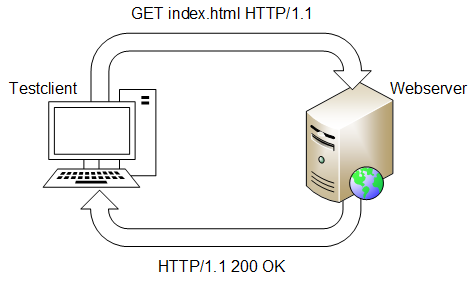
\includegraphics[scale=1]{figures/httpget.png}

Der Webservice kann durch mehrere Komponenten beinträchtigt werden. Meistens beitzt man eine 3-Tier Architektur und bei jedem Tier kann es zu Fehlern kommen. Daher ist es sehr schwer herauszufinden, wo der Fehler entstanden ist. So kann man mit einer falschen Firewallregeln den Webservice unerreichbar machen.

\subsubsection{Porterreichbarkeit}
Sobald man in den oberen OSI-Layern angekommen ist, benötigt man einen Port. Daher ist es wichtig, dass die benötigten Ports des jeweiligen Services auch erreichbar sind. Bei jeder 
\end{document}

